%!TEX root = ../report.tex
\documentclass[../report.tex]{subfiles}

\begin{document}
\section{Methodology}
\label{sec:methodology}

\subsection{LLM Cognition}
The robot's cognitive architecture is built around a large language model (LLM) that serves as the central decision-making component. This LLM-based approach allows the robot to process natural language instructions, reason about its environment, and select appropriate actions through a tool-calling interface.

At the core of the robot's cognition system is its memory architecture, which consists of three distinct components that mirror cognitive processes: episodic memory, working memory, and action execution. The episodic memory is implemented using ChromaDB, a vector database that stores the robot's past experiences as embeddings. This allows the robot to perform similarity searches through its previous interactions, retrieving relevant experiences that can inform current decision-making processes. When the robot encounters a new task, it can query this episodic memory to find similar past scenarios and adapt successful strategies from those experiences.

The working memory of the system is represented by the LLM's context, which dynamically incorporates environmental information, task descriptions, and the robot's internal reasoning. This working memory is updated at each step with information such as the current perceptual data from the environment and results of actions or tool calls ensuring that the robot's decisions are based on the most recent state of the world.

The action execution module consists of a toolkit of functions that translate high-level decisions into concrete robotic actions. These tools include navigation, manipulation, memory operations, and reasoning capabilities through a scratchpad mechanism. The perception components gather information about the robot's current location, nearby objects, and environmental layout, which is then integrated into the working memory to inform decision-making.

This cognitive architecture enables the robot to combine long-term learning from past experiences with immediate environmental awareness, allowing for adaptive and context-aware behavior in complex environments.

\subsection{Simulation}
The agent and its environment were simulated using the PyBullet physics engine. As PyBullet is a Python module, its functionality can be directly integrated in any Python script. This allows precise control over the simulation and its interaction with external tool calls. PyBullet also comes with methods to create custom objects as well as a fully implemented robotic arm, the KUKA iiwa model. These methods and the KUKA iiwa robotic arm were used to create the agent's embodiment and the environment it can act in.

The agent's body is modeled as a mobile manipulator, consisting of a square omnidirectional base and a 7-DoF robotic arm derived from the KUKA iiwa model.
To increase maneuverability, the rotational joint limits of the arms joint connecting the base to the arm were disabled, enabling full 360° reach around the base. A fully articulated gripper was not implemented. Instead, grasping and placing were simplified by attaching objects directly to the end-effector when within a predefined proximity threshold, and detaching them at the desired placement location. Figure \ref{fig:agent} depicts the agent.

\begin{figure}[h!]
	\centering
	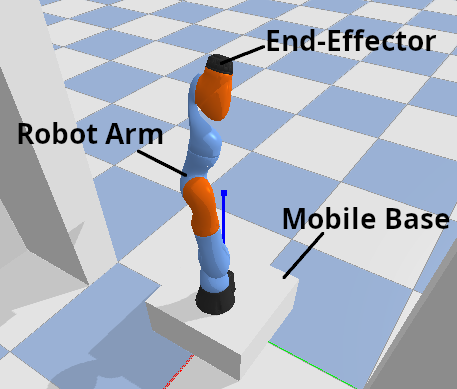
\includegraphics[width=0.45\textwidth]{figures/agent.png}
	\caption{The simulated mobile manipulator consisting of a square omnidirectional base and a 7-DoF arm.}
	\label{fig:agent}
\end{figure}

The environment was designed as a simplified two-room household, comprising a kitchen and a living room. The kitchen contains a three-layer shelf and a table, both capable of supporting objects. The living room contains a television placed on a table. The two rooms are connected by a hallway. Figure \ref{fig:environment} shows the environment and the semantic map used for navigation. The green dots are locations the agent can navigate to via the connected lines.

\begin{figure}[h!]
	\centering
	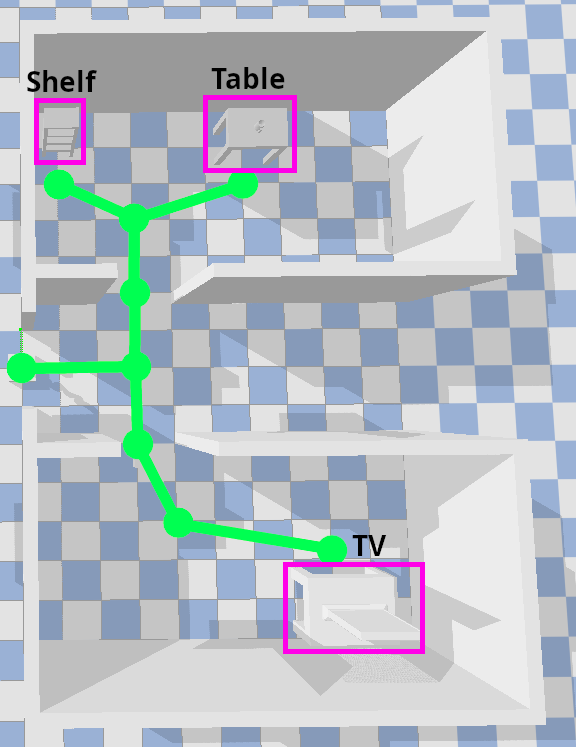
\includegraphics[width=0.45\textwidth]{figures/environment.png}
	\caption{The simulated household environment and its semantic map representation consisting of a kitchen, a living room, and a connecting hallway.}
	\label{fig:environment}
\end{figure}

To interact with the environment and its objects, the agent was equipped with several tool functions, each exposed through a tool-calling interface with text-based status responses. The implemented tools are summarized below:
\begin{itemize}
	\item \textbf{Look around:} Returns the agent's location on a semantic map of the environment, as well as a list of objects detected in proximity of the agent and where these objects are placed.
	\item \textbf{Search memory:} The agent queries its episodic memory to gain information from prior executions of tasks. It returns relevant past experiences that might help with the current task.
	\item \textbf{Move to:} Executes navigation to a goal location on the semantic map. Path planning is performed using the A* algorithm; if a valid path is found, the agent follows it until the goal is reached. If no path is available, the tool reports failure.
	\item \textbf{Grab:} Moves the robot arm toward a specified target object. If the end-effector reaches within a proximity threshold, the object is attached to the arm, and the tool reports success. Failure is reported if the target object does not exist, is out of reach, or if the agent is already holding an object.
	\item \textbf{Place:} Allows the agent to release the currently held object at a specified location. Placement succeeds if the end-effector reaches the designated location, the location is unoccupied, and the agent is holding an object. Otherwise, the tool reports failure, specifying the violated condition.
	\item \textbf{Add to scratchpad:} The agent can write down thoughts and plans for reasoning and reflection. This allows the agent to plan, reason and organize its thoughts before taking action.
	\item \textbf{View scratchpad:} The agent can view the current contents of its scratchpad, which contains previous thoughts and plans joined as paragraphs.
	\item \textbf{End task:} The agent ends the current task with a status report, including whether it succeeded or failed, and provides a detailed summary of actions taken during the task execution.
\end{itemize}

\end{document}
